El proceso de creación de nuestra API inicia con la configuración del entorno de desarrollo, utilizando Python, un lenguaje de programación ampliamente reconocido, junto con diversas bibliotecas especializadas. Inicialmente, se importa Flask, una herramienta eficaz para la creación de aplicaciones web, que facilita la gestión de solicitudes a través de internet. Además, se integra TensorFlow, una biblioteca de vanguardia para el manejo de aprendizaje automático, que será fundamental en la utilización de un modelo de clasificación, es decir, un sistema entrenado para categorizar datos.

El modelo de clasificación se almacena en un archivo con formato .h5, que preserva íntegramente la estructura y datos del modelo. Este se carga mediante TensorFlow, preparando el modelo para realizar predicciones efectivas.

Adicionalmente, la API opera con dos archivos en formato JSON, \textquotedblleft method\_to\_int.json\textquotedblright y \textquotedblleft channel\_to\_int.json\textquotedblright. Este formato estructura la información de manera clara, facilitando su interpretación tanto por humanos como por sistemas automatizados. Los archivos contienen mapeos, similares a diccionarios, que permiten convertir texto en valores numéricos, adaptándose a las limitaciones del modelo que no procesa texto directamente.

Posteriormente, se define una ruta especial \textquotedblleft\/predict\textquotedblright en la aplicación Flask. Las solicitudes recibidas en esta dirección son procesadas en formato JSON, utilizando los mapeos mencionados y ajustando la longitud de los datos con \textquotedblleft pad\_sequences\textquotedblright para cumplir con las especificaciones del modelo.

Los datos procesados se introducen en el modelo de clasificación para su análisis, generando predicciones sobre la categoría a la que pueden pertenecer. El modelo proporciona estimaciones con un grado de confianza asociado a cada predicción.

Finalmente, la API responde a las solicitudes, entregando en formato JSON la categoría predicha junto con la confianza del modelo en dicha predicción, asegurando una interpretación y uso sencillos y eficientes.

\begin{figure}[H]
    \begin{minipage}[t]{0.9\textwidth}
        \caption{Código creación API}
        \label{API_creation}        
    \end{minipage}

    \vspace{10pt}

    \begin{minipage}[b]{1\textwidth}
        \centering
        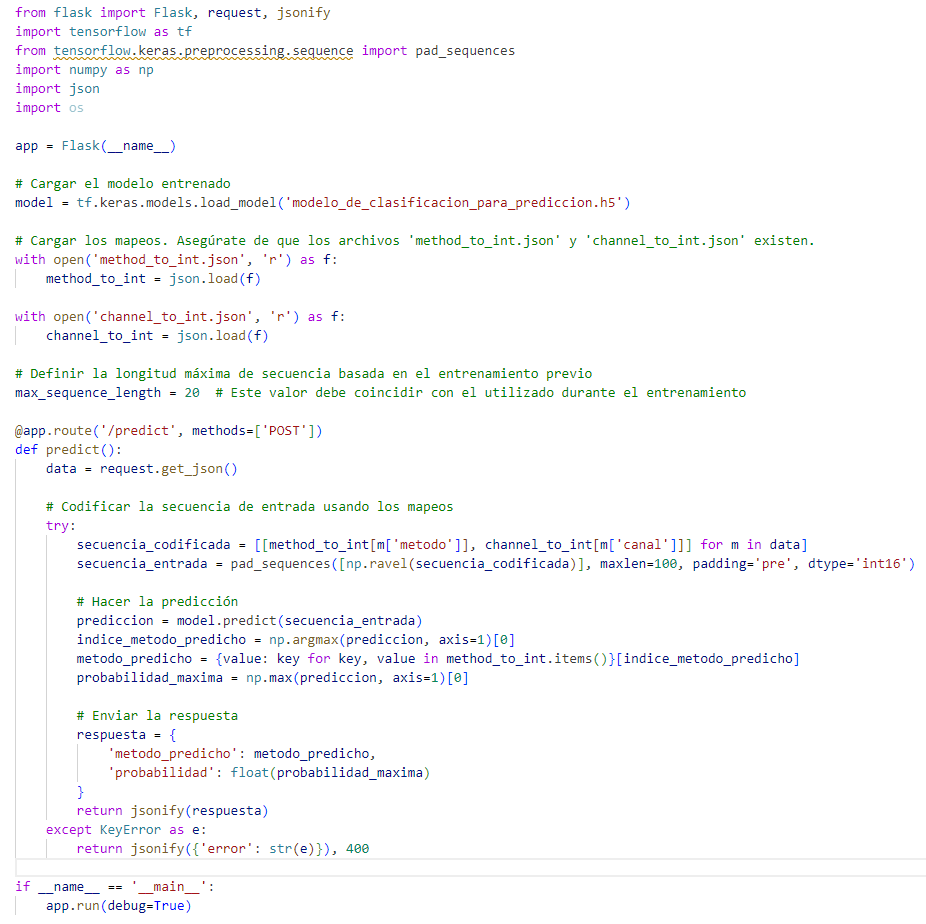
\includegraphics[width=\textwidth]{img/SS_API.png}        
    \end{minipage}

    \begin{minipage}[t]{0.9\textwidth}
        Fuente: Elaboración propia.
    \end{minipage}
\end{figure}

Para garantizar un funcionamiento óptimo, se ejecuta la aplicación Flask en un modo de "depuración", que facilita la identificación y resolución rápida de problemas, mejorando así la estabilidad y fiabilidad del sistema. Además de contar con códigos de estatus para saber como va funcionando la API, el código 200 representa el correcto funcionamiento y cuando se presenta algún error en el ingreso de parámetros la API no funcionara y se desplegara el código 400 que representa el incorrecto funcionamiento, junto a la descripción de la causa del error.

\begin{figure}[H]
    \begin{minipage}[t]{0.9\textwidth}
        \caption{Prueba de funcionamiento API de predicción en Postman}
        \label{API_test}        
    \end{minipage}

    \vspace{10pt}

    \begin{minipage}[b]{1\textwidth}
        \centering
        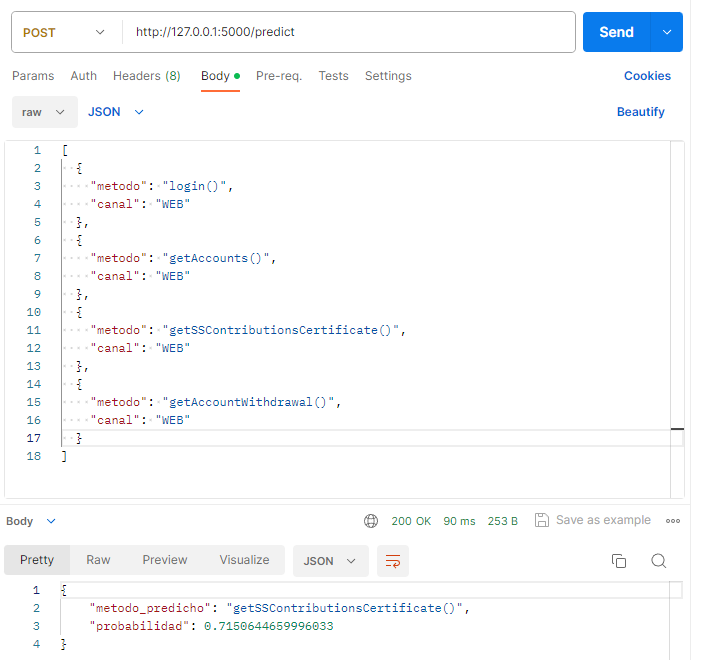
\includegraphics[width=\textwidth]{img/postman.png}        
    \end{minipage}

    \begin{minipage}[t]{0.9\textwidth}
        Fuente: Elaboración propia.
    \end{minipage}
\end{figure}

